\documentclass[10pt,conference]{IEEEtran}
\usepackage{graphicx}
\usepackage{cite}
\usepackage{url}

\title{AI-Assisted Mixed-Signal Physical Design Flow}
\author{\IEEEauthorblockN{Shravani Bai K V}
\IEEEauthorblockA{Week 1 Task Report -- Mixed-Signal Physical Design}}
\date{}

\begin{document}
\maketitle

\begin{abstract}
This report summarizes a Week 1 study of the \texttt{vsdmixedsignalflow} repository, which demonstrates mixed-signal physical design using OpenLane, SKY130, LEF/LIB/Verilog inputs, analog macro integration, placement, PDN generation, routing, DRC, and Magic layout viewing. AI tools were used to structure prompts, organize debugging, and prepare documentation. All suggestions were verified through terminal output, layout views, and flow results.
\end{abstract}

\begin{IEEEkeywords}
Mixed-signal physical design, OpenLane, SKY130, AI-assisted debugging, analog macro, physical verification
\end{IEEEkeywords}

\section{Objective}
The objective was to understand the fundamentals of mixed-signal physical design and reproduce similar results to the \texttt{praharshapm/vsdmixedsignalflow} repository. The work was divided into repo understanding, tool setup, input study, macro checking, OpenLane configuration, flow execution, error fixing, and documentation.

\section{Reference Repo Summary}
The repository implements an OpenLane flow for the digital top design \texttt{design\_mux}, integrating the analog macro \texttt{AMUX2\_3V}. The macro is represented using LEF, LIB, and Verilog views. LEF provides macro size, pins, routing layers, and obstructions; LIB provides timing/power abstraction; and blackbox Verilog preserves the analog macro during synthesis. OpenLane then performs synthesis, floorplanning, placement, PDN generation, routing, Magic DRC, and final layout generation.

\section{AI Workflow}
ChatGPT was used to create step-by-step prompts for understanding the repo, checking SKY130/OpenLane setup, explaining LEF/LIB/Verilog roles, validating macro pins, reviewing configuration, running flow stages, debugging DRC/DEF errors, and writing the report. Each AI suggestion was treated as guidance and verified through terminal output, Magic layout views, and screenshots.

\section{Experiments}
The \texttt{AMUX2\_3V} macro was inspected in Magic using SKY130A technology files. The integrated \texttt{design\_mux} layout was also reproduced through the OpenLane/LibreLane flow. Early runs exposed RTL and abstraction issues, including pin-access failures, disconnected macro pins, and power-grid connectivity warnings. After iterative fixes to the macro abstraction and flow configuration, the design progressed through routing and produced a final GDS.

\section{Results and Observations}

The \texttt{design\_mux} mixed-signal design was synthesized, placed, routed, and streamed out to GDS using LibreLane/OpenROAD with the SKY130 PDK. Several issues were encountered during reproduction, including Verilator compatibility problems, macro pin-access failures, and power-pin connectivity warnings associated with the \texttt{AMUX2\_3V} macro. After iterative fixes, the flow reached GDS generation, and Magic reported \texttt{DRC=0}. Figure~\ref{fig:gds_layout} shows the final layout. The reproduced flow was largely consistent with the reference repository.

\begin{figure}[t]
\centering
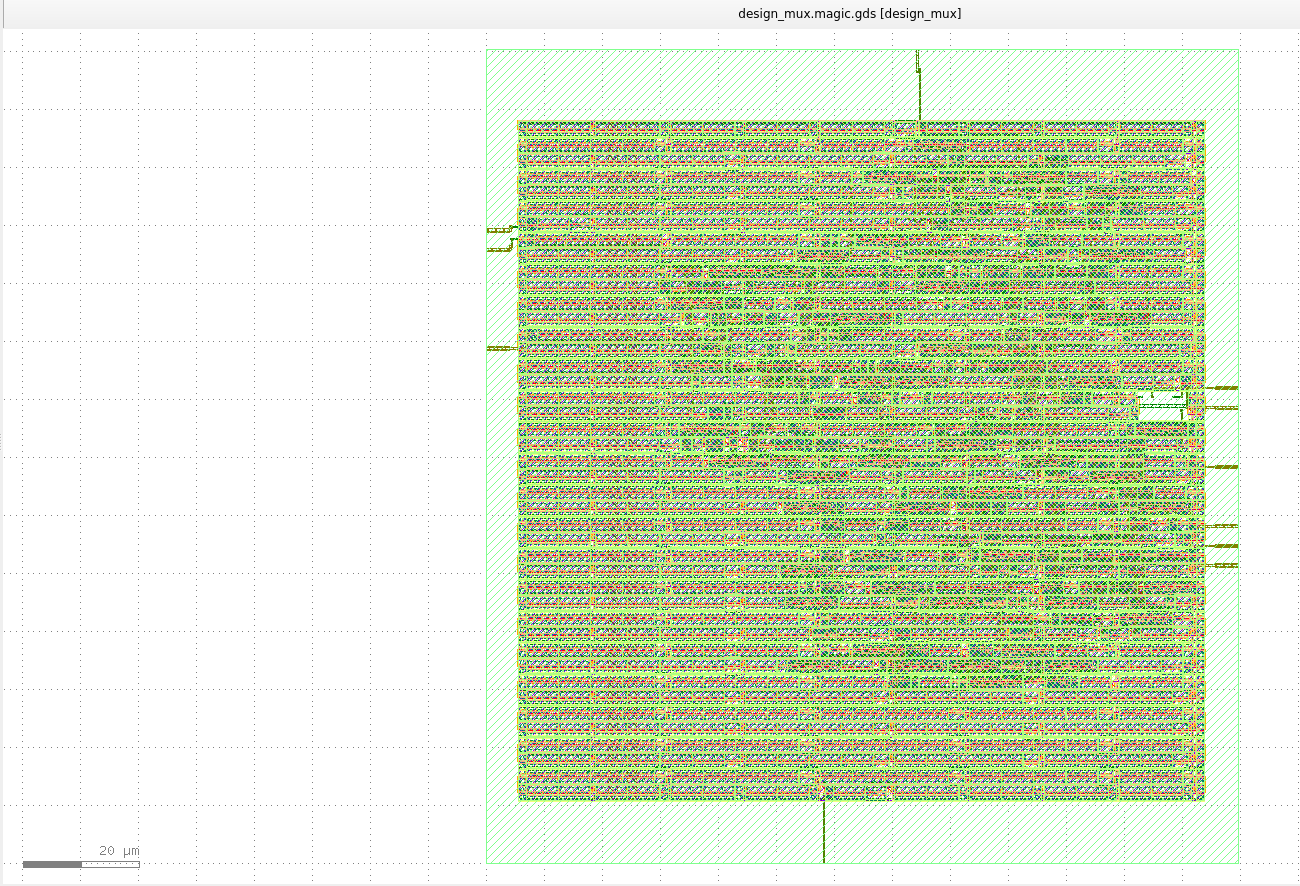
\includegraphics[width=\columnwidth]{task1_gds}
\caption{Final GDS layout of the reproduced \texttt{design\_mux} design.}
\label{fig:gds_layout}
\end{figure}

\section{Challenges and Next Steps}

The primary challenge was debugging macro abstraction and power-connectivity issues. Future work includes resolving the remaining signoff warnings.

\section{Conclusion}

This work successfully reproduced a mixed-signal RTL-to-GDS flow using LibreLane/OpenROAD and SKY130. The final design reached GDS generation and achieved a \texttt{DRC=0} Magic result, providing practical insight into mixed-signal physical-design integration and verification.

\begin{thebibliography}{3}
\bibitem{repo} P. M., ``vsdmixedsignalflow,'' GitHub. Available: \url{https://github.com/praharshapm/vsdmixedsignalflow}

\bibitem{openlane}
The OpenLane Project, ``OpenLane Documentation.'' Available:
\url{https://openlane.readthedocs.io}

\bibitem{sky130}
SkyWater Technology and Google, ``SKY130 Open Source PDK.'' Available:
\url{https://github.com/google/skywater-pdk}

\end{thebibliography}


\end{document}
